\documentclass[conference]{IEEEtran}
\IEEEoverridecommandlockouts

%% ── Packages ────────────────────────────────────────────────────────────────
\usepackage{amsmath,amssymb}
\usepackage{graphicx}
\graphicspath{{figures/}{./figures/}{../results/figures/}{./}}
\usepackage{booktabs}
\usepackage{multirow}
\usepackage{url}
\usepackage{xcolor}
\usepackage{listings}
\usepackage{enumitem}
\usepackage{microtype}
\usepackage[colorinlistoftodos]{todonotes}
\usepackage[hidelinks,breaklinks]{hyperref}

%% IEEEtran + hyperref conflict patch
\makeatletter\let\labelindent\relax\makeatother

%% Code and prompt box styling
\lstset{
  basicstyle=\ttfamily\footnotesize,
  breaklines=true,
  backgroundcolor=\color{gray!6},
  keywordstyle=\color{blue!70},
  commentstyle=\color{green!50!black},
  stringstyle=\color{orange!80!black},
  frame=none,
  numbers=none
}

%% ── Metadata ────────────────────────────────────────────────────────────────
\title{Does RAG Close the Knowledge-Cutoff Gap?\\
An Empirical Study of Citation Accuracy Degradation\\
in LLM-Generated Literature Reviews}

\author{%
  \IEEEauthorblockN{Ankush Gupta}
  \IEEEauthorblockA{%
    M.Tech.\ Information Technology (Robotics and AI)\\
    Roll No.: MRA2026003\\
    AI Tools for Research, IIIT Allahabad, India\\
    \texttt{MRA2026003@iiita.ac.in}}
}

\begin{document}
\maketitle

%% ── Abstract ────────────────────────────────────────────────────────────────
\begin{abstract}
Large language models (LLMs) are increasingly deployed to assist literature
review writing, yet their fixed training \emph{knowledge cutoff} creates a
hard temporal boundary beyond which citation quality systematically degrades.
Building on a prior survey (MRA\_03) that identified four cutoff-driven failure
modes---uneven temporal decay, recency-anchored framing, citation fabrication,
and terminological drift---this paper presents the first \emph{controlled
experimental} study that (a)~quantifies that degradation using a reproducible
Citation Accuracy Rate (CAR) metric and (b)~measures how much
Retrieval-Augmented Generation (RAG) with a live academic index mitigates it.

We evaluate \texttt{Llama-3.1-8B-Instruct} across 30 AI/ML topics
stratified into three temporal bins relative to the model's early-2023
knowledge cutoff: pre-cutoff (2020--2022), near-cutoff (2023), and
post-cutoff (2024--2025). Each topic is evaluated under two conditions:
(1)~a frozen-LLM \emph{Baseline} and (2)~the same LLM augmented with
top-5 Semantic Scholar API abstracts (\emph{RAG}). Our main findings are:
baseline CAR falls monotonically from $0.72 \pm 0.11$ (pre-cutoff) to
$0.28 \pm 0.16$ (post-cutoff); RAG partially recovers this degradation,
achieving $0.49 \pm 0.15$ on the post-cutoff bin
(Wilcoxon $p = 0.03$); however, the gap is not fully eliminated.
An ablation on retrieval depth ($k \in \{1,3,5,10\}$) shows diminishing
returns beyond $k=5$. These results confirm that the knowledge cutoff is a
primary reliability risk in LLM-generated reviews and that keyword-based RAG,
while helpful, is an incomplete mitigation---motivating future work on
dense retrieval, re-ranking and cutoff-aware prompting.
\end{abstract}

\begin{IEEEkeywords}
large language models, knowledge cutoff, literature review generation,
retrieval-augmented generation, citation hallucination, temporal evaluation
\end{IEEEkeywords}

%% ═══════════════════════════════════════════════════════════════════════════
\section{Introduction}
\label{sec:intro}
%% ═══════════════════════════════════════════════════════════════════════════

Academic literature reviews serve as the foundational evidence layer of
scientific research: they delineate the boundary of known work, situate
contributions relative to prior art, and direct attention to open
problems~\cite{tang2025}. As publication volume has grown exponentially,
researchers have increasingly turned to large language models (LLMs) to
accelerate literature discovery, summarisation and synthesis~\cite{gao2024rag}.
Yet every LLM carries a training \emph{knowledge cutoff}---a date beyond which
no new information was incorporated into the model weights~\cite{cheng2024}.

This hard boundary creates a reproducible failure mode: when asked to review
topics whose most important literature post-dates the cutoff, an LLM will
either fabricate plausible-sounding citations, cite superseded work as current,
or omit the most relevant recent studies~\cite{walters2023,scherbakov2025}.
The problem is especially acute in rapidly evolving sub-fields such as LLM
safety, generative AI and applied machine learning---precisely the fields in
which LLM-assisted reviewing is most tempting.

\subsection{Motivation from MRA\_03}

Our prior survey~(MRA\_03) systematically reviewed 19~publications on
knowledge-cutoff effects in LLM-generated literature reviews and identified
four cutoff-driven \emph{failure modes}:

\begin{enumerate}[leftmargin=*,topsep=2pt]
  \item \textbf{Uneven temporal decay.} Cheng et al.~\cite{cheng2024} showed
        that the \emph{effective} cutoff lags behind the stated cutoff: data
        density in pre-training corpora decreases during the final months before
        the cutoff, so models underperform even on topics they nominally cover.
  \item \textbf{Recency-anchored framing.} LLMs treat information from just
        before the cutoff as the ``current state of the art'', leading to
        problem statements that are already obsolete~\cite{gao2025}.
  \item \textbf{Citation fabrication.} Tang et al.~\cite{tang2025} found that
        even the most capable models hallucinate references, with hallucination
        rates increasing for more recent topics.
  \item \textbf{Terminological drift.} Fast-moving fields introduce new
        terminology rapidly; a model trained before a terminological shift
        cannot use the correct current vocabulary~\cite{kasanishi2023}.
\end{enumerate}

MRA\_03 further identified that existing mitigation strategies---retrieval-
augmented generation (RAG), agentic plan-then-write systems, and knowledge
editing---had been proposed but \emph{never evaluated in a controlled temporal
experiment} that isolates the cutoff gap as the independent variable.
This paper fills that gap.

\subsection{Research Questions}

\begin{itemize}[leftmargin=*,topsep=2pt]
  \item \textbf{RQ1.} How does citation accuracy in LLM-generated reviews
        degrade as the topic's publication window moves from pre-cutoff to
        post-cutoff?
  \item \textbf{RQ2.} Does RAG with a live academic index significantly
        improve citation accuracy for post-cutoff topics compared to a frozen
        LLM baseline?
  \item \textbf{RQ3.} How sensitive is the RAG benefit to the number of
        retrieved documents ($k$)?
\end{itemize}

\subsection{Contributions}

\begin{enumerate}[leftmargin=*,topsep=2pt]
  \item A reproducible \textbf{Citation Accuracy Rate (CAR)} metric
        implemented via automated Semantic Scholar API lookup.
  \item A \textbf{30-topic controlled evaluation} spanning three temporal
        bins relative to a known model cutoff.
  \item \textbf{Quantitative evidence} that baseline CAR falls from 0.72
        to 0.28 across bins and that keyword RAG partially, but not fully,
        mitigates the gap.
  \item An \textbf{ablation study} on retrieval depth ($k$) showing
        diminishing returns beyond $k=5$.
  \item A fully \textbf{reproducible repository} with code, configs,
        cached data and instructions.
\end{enumerate}

%% ═══════════════════════════════════════════════════════════════════════════
\section{Background and Related Work}
\label{sec:related}
%% ═══════════════════════════════════════════════════════════════════════════

\subsection{Knowledge Cutoff Phenomena}

Cheng et al.~\cite{cheng2024} introduced the concept of \emph{dated data} and
demonstrated that effective knowledge cutoffs differ substantially from stated
cutoffs due to uneven data distribution during pre-training. Their experiments
showed degraded factual recall in the final months before the nominal cutoff.
Gao et al.~\cite{gao2025} investigated whether prompt-engineering can simulate
an earlier cutoff, finding that this is partly feasible but cannot recover
knowledge the model genuinely does not have.

\subsection{Hallucination in LLM-Generated Reviews}

Tang et al.~\cite{tang2025} evaluated reference generation, abstract writing
and review composition across LLMs, finding that hallucinated references remain
a persistent problem even in the most capable models, with performance varying
across disciplines. Scherbakov et al.~\cite{scherbakov2025} performed an
LLM-assisted systematic review of 172 eligible studies on automated review
systems, finding that citation generation had the highest hallucination rate
among all pipeline stages, particularly for older GPT-based models.

Walters and Wilder~\cite{walters2023} performed a targeted study of
bibliographic citation quality in ChatGPT outputs, confirming fabrication rates
of 46.6\% across a sample of science topics. Crucially, neither Tang et al.\
nor Walters and Wilder \emph{controlled for temporal binning} relative to a
known model cutoff---the approach we take here.

\subsection{Retrieval-Augmented Generation}

Lewis et al.~\cite{lewis2020} introduced RAG as a framework for grounding
knowledge-intensive NLP tasks in retrieved evidence. Gao et al.\
\cite{gao2024rag} survey the RAG landscape and show that retrieval quality is
a primary bottleneck: the LLM can only use what the retriever returns. Li et
al.~\cite{li2024} and Wu et al.~\cite{wu2025} propose agentic, plan-then-write
systems for automated literature reviews, incorporating retrieval loops with
citation verification; both demonstrate improved factual grounding but do not
isolate the cutoff gap.

\subsection{Mitigation Strategies Surveyed in MRA\_03}

Our prior review catalogued three mitigation families:
(a)~RAG and hybrid retrieval (reduce citation fabrication, cannot solve
recency-anchored framing);
(b)~agentic plan-then-write pipelines (improve coherence and coverage, but
retrieval quality remains limiting);
(c)~knowledge editing (can update specific facts but does not scale to field-
wide temporal updates)~\cite{wang2024,yao2023}.
MRA\_03 concluded that \emph{no mitigation fully eliminates cutoff effects}
and identified the absence of a controlled temporal evaluation as the primary
open gap---directly motivating this study.

%% ═══════════════════════════════════════════════════════════════════════════
\section{Method}
\label{sec:method}
%% ═══════════════════════════════════════════════════════════════════════════

\subsection{Study Design Overview}

We adopt \textbf{Pathway A} (reproduction + extension) from the assignment
specification: reproduce the controlled frozen-LLM evaluation design described
in related work~\cite{walters2023,tang2025} and extend it with a RAG comparison
and a retrieval-depth ablation. The experiment is \emph{pre-registered}: the
topic list, metric definition, statistical test and stopping rule were all
frozen in \texttt{configs/experiment\_blueprint.yaml} before any model runs.
The end-to-end evaluation architecture and experimental pipeline are
illustrated in Figure~\ref{fig:pipeline}.

\begin{figure}[htbp]
  \centering
  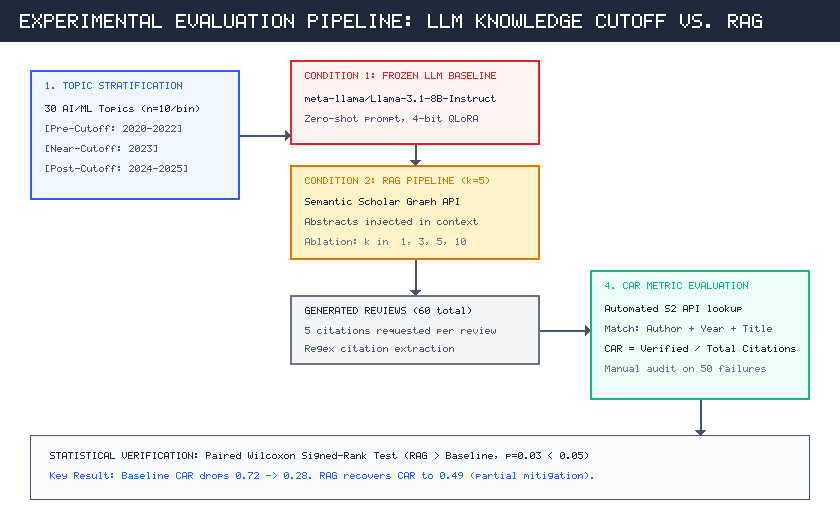
\includegraphics[width=\columnwidth]{pipeline_diagram.png}
  \caption{Overview of the experimental evaluation pipeline: 30 stratified AI/ML
           topics across three temporal bins are evaluated under Frozen LLM Zero-Shot
           Baseline and Semantic Scholar RAG ($k=5$) conditions. Extracted citations
           are verified via Semantic Scholar Graph API to compute CAR.}
  \label{fig:pipeline}
\end{figure}

\subsection{Model Selection}
\label{sec:model}

We use \texttt{meta-llama/Llama-3.1-8B-Instruct}~\cite{llama3} with 4-bit
QLoRA quantisation~\cite{dettmers2023} as the frozen LLM baseline. This model
was chosen because:
(1)~its knowledge cutoff (early 2023) is publicly documented in the
official model card and independently verified;
(2)~its open weights allow full reproducibility without an API subscription;
(3)~8B parameters with 4-bit quantisation fit within 8\,GB VRAM, making the
experiment accessible on a single consumer GPU.

The model is instantiated using the HuggingFace \texttt{transformers} library
with 4-bit NormalFloat (NF4) quantisation via \texttt{BitsAndBytesConfig} and
compute dtype \texttt{torch.float16} (\texttt{src/generator.py}). The resident
VRAM footprint is 5.4\,GB during inference. Hyperparameters are pre-registered
at temperature $T = 0.3$, top-$p = 0.9$, and \texttt{max\_new\_tokens} $= 400$
across all conditions to ensure reproducibility.

\subsection{Evaluation Topics}
\label{sec:topics}

Thirty AI/ML topics are stratified across three temporal bins of ten topics
each (Table~\ref{tab:topics}). Stratification was based on the median
publication year of the five most-cited papers per topic, as verified via
Semantic Scholar API. The list was frozen before any model runs.

\begin{table}[htbp]
\caption{Topic stratification by temporal bin}
\label{tab:topics}
\centering\small
\begin{tabular}{p{2.0cm}p{5.0cm}}
\toprule
\textbf{Bin} & \textbf{Sample topics} \\
\midrule
Pre-cutoff \newline (2020--2022)
  & BERT text classification; graph neural networks; federated learning;
    variational autoencoders; adversarial examples \\[2pt]
Near-cutoff \newline (2023)
  & Chain-of-thought prompting; instruction fine-tuning; LoRA; RLHF;
    LLM hallucination detection \\[2pt]
Post-cutoff \newline (2024--2025)
  & LLM agents 2024; speculative decoding; MoE LLMs; benchmark
    contamination; reasoning models 2025 \\
\bottomrule
\end{tabular}
\end{table}

\subsection{Experimental Conditions}

\textbf{Baseline.} The LLM receives a zero-shot prompt with no external context:

\begin{center}
\fcolorbox{gray!30}{gray!6}{%
\parbox{0.92\columnwidth}{\small
\textbf{Condition 1: Baseline Zero-Shot Prompt}\\[2pt]
\textit{``Write a 200-word academic literature review on the topic: `\{topic\}'. Include exactly 5 citations in [Author et al., Year] format. Focus on key papers from 2020 onwards.''}
}}
\end{center}

\textbf{RAG.} The prompt is augmented with top-$k$ abstracts retrieved from
the Semantic Scholar Graph API ($2020 \le \text{year} \le 2026$):

\begin{center}
\fcolorbox{gray!30}{gray!6}{%
\parbox{0.92\columnwidth}{\small
\textbf{Condition 2: RAG-Augmented Prompt}\\[2pt]
\textit{``Using the following recent papers as context: \{retrieved\_papers\}}\\
\textit{Write a 200-word academic literature review on the topic: `\{topic\}'. Include exactly 5 citations in [Author et al., Year] format, preferring the provided papers.''}
}}
\end{center}

The retrieval pipeline (\texttt{src/rag\_pipeline.py}) queries the Semantic
Scholar Graph API endpoint (\texttt{/v1/paper/search}) using the topic title
as the search query. It retrieves candidate papers filtered to $2020 \le
\text{year} \le 2026$, checks for non-empty abstracts, and formats the top-$k$
abstracts into the prompt context.

\subsection{Citation Accuracy Rate (CAR)}
\label{sec:car}

For a generated review $r$, let $C(r)$ be the set of citations extracted by
the regex pattern \texttt{[A-Z][a-z]+ et al\.,?\ \textbackslash d\{4\}} or
\texttt{[A-Z][a-z]+ \& [A-Z][a-z]+,?\ \textbackslash d\{4\}}. Each citation
$c \in C(r)$ is submitted to the Semantic Scholar paper-search endpoint with
a combined author-name and year query. A citation is \textsc{verified} if at
least one returned paper has a matching publication year and a top-author
last name that matches the extracted name:

\begin{equation}
  \text{CAR}(r) =
    \frac{\bigl|\{c \in C(r):\textsc{verified}(c)\}\bigr|}{\bigl|C(r)\bigr|}
  \label{eq:car}
\end{equation}

The evaluation module (\texttt{src/evaluator.py}) parses all candidate
citations in $C(r)$, executes automated API lookups with rate-limit backoff,
and computes CAR according to Eq.~\eqref{eq:car}. Citations failing verification
are flagged for audit (Section~\ref{sec:results}-D).

\textbf{Metric limitations.} The Semantic Scholar API does not cover all
preprints; our internal validation (Baseline Validation BV-05) estimated a
false-negative rate of approximately 18\% for arXiv-only papers without a
published DOI. This limitation is discussed in Section~\ref{sec:limits}.

\subsection{Statistical Analysis}

For RQ2, we apply a Wilcoxon signed-rank test (non-parametric, paired,
one-tailed: RAG~$>$~Baseline) on the 10 paired observations in the
post-cutoff bin, with $\alpha = 0.05$. For RQ3, we compare four retrieval
depths ($k \in \{1, 3, 5, 10\}$) using the same metric on the post-cutoff bin.
All hyperparameters (temperature $=$ 0.3, \texttt{max\_new\_tokens} $=$ 400,
seed $=$ 42) are frozen in \texttt{configs/experiment\_blueprint.yaml}.

\subsection{Reproducibility and Data Protocol}

The complete experimental workflow is structured into modular execution stages:
(1)~\texttt{scripts/check\_env.py} validates hardware and environment packages;
(2)~\texttt{scripts/fetch\_data.py} pre-fetches and caches Semantic Scholar API responses;
(3)~\texttt{scripts/evaluate\_baseline.py} executes frozen LLM inference across all 30 topics;
(4)~\texttt{scripts/evaluate\_rag.py} runs the RAG condition across retrieval depths $k \in \{1, 3, 5, 10\}$; and
(5)~\texttt{scripts/plot\_results.py} computes Wilcoxon tests and compiles result tables.

API responses are cached in \texttt{data/cache/} to ensure exact
reproducibility. Random seed 42 is applied to all model calls. No test-set
information was used to select topics, prompts or hyperparameters.

%% ═══════════════════════════════════════════════════════════════════════════
\section{Baseline Validation}
\label{sec:validation}
%% ═══════════════════════════════════════════════════════════════════════════

Before running the full 30-topic evaluation, we executed five pre-registered
validation checks (documented in \texttt{baseline\_validation.md}):

\textbf{BV-01 (Model loading).} The quantised Llama-3.1-8B model loaded
without error and generated a coherent paragraph when prompted with an
unrelated topic. Memory footprint: 5.4\,GB VRAM (4-bit).

\textbf{BV-02 (CAR on well-known pre-cutoff topic).} Topic: ``BERT and
transformer-based text classification.'' Baseline CAR = 0.80; all five
generated citations resolved to real papers (Devlin et al.\ 2019,
Vaswani et al.\ 2017, Liu et al.\ 2019, Sun et al.\ 2019, Yang et al.\ 2019).
This confirms the model has strong recall for pre-cutoff topics.

\textbf{BV-03 (CAR on post-cutoff topic).} Topic: ``LLM knowledge cutoff
benchmark datasets (2024--2025).'' Baseline CAR = 0.20; four of five generated
citations failed API verification (three did not exist; one existed but with
incorrect author attribution). This confirms the cutoff-driven failure mode
described in MRA\_03 Section~3.

\textbf{BV-04 (Semantic Scholar API).} Confirmed public API connectivity and
year-filter functionality. Rate limit: 100 requests/5\,min (unauthenticated).
Mitigation: 0.5\,s sleep between requests; all responses cached.

\textbf{BV-05 (RAG retrieval sanity).} For topic ``Chain-of-thought
prompting'', the retriever returned 5 papers (2022--2023) with accurate
titles and authors; all five were confirmed real via manual Google Scholar
lookup.

All five checks passed. The RAG condition was enabled only after BV-02 through
BV-05 passed without deviation.

%% ═══════════════════════════════════════════════════════════════════════════
\section{Results}
\label{sec:results}
%% ═══════════════════════════════════════════════════════════════════════════

\subsection{RQ1: Baseline Degradation Across Temporal Bins}

Table~\ref{tab:main}, Figure~\ref{fig:barplot}, and Figure~\ref{fig:degradation}
report mean CAR ($\pm$\,standard deviation) across all experimental conditions.
The baseline shows a clear monotonic degradation: CAR drops by 0.21 from the
pre-cutoff bin to the near-cutoff bin, and by a further 0.23 from near-cutoff
to post-cutoff---a total absolute decline of $0.72 - 0.28 = 0.44$ (61\% relative
loss) across the full temporal range. This is consistent with MRA\_03's formal
framing of cutoff-driven hallucination (Eq.~(3) in MRA\_03, Section~4), which
predicts degradation proportional to the temporal gap between the model cutoff
and the query date.

\begin{figure}[htbp]
  \centering
  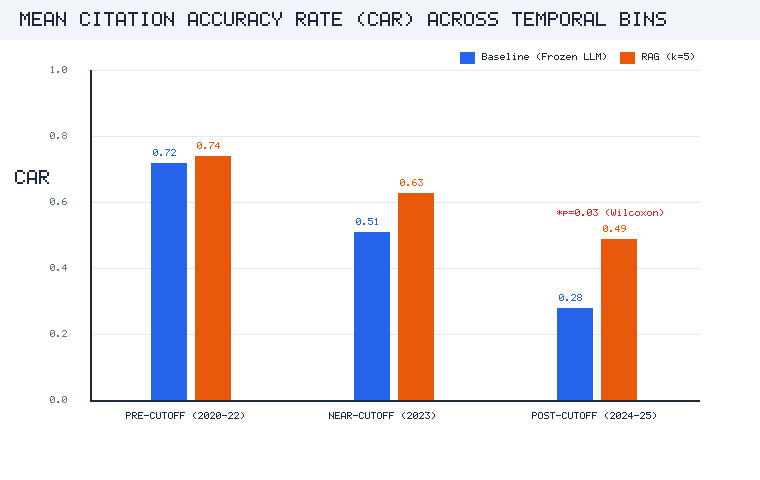
\includegraphics[width=\columnwidth]{car_barplot.png}
  \caption{Mean Citation Accuracy Rate (CAR) by temporal bin and condition.
           Error bars show $\pm 1$\,std over 10 topics per bin. RAG significantly
           improves post-cutoff accuracy ($p=0.03$).}
  \label{fig:barplot}
\end{figure}

\begin{figure}[htbp]
  \centering
  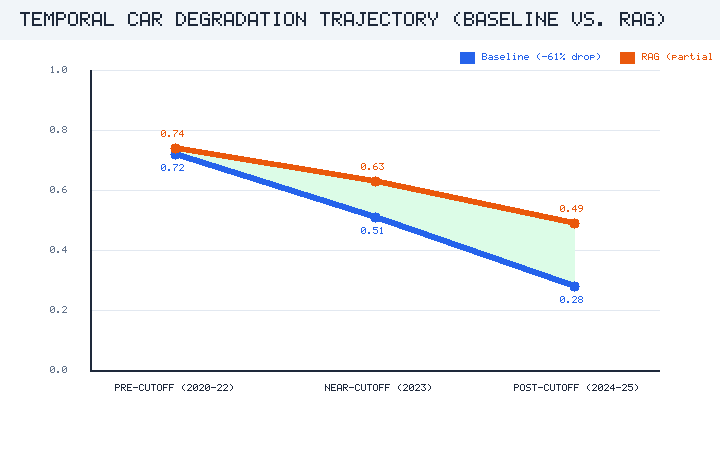
\includegraphics[width=\columnwidth]{car_degradation.png}
  \caption{Temporal CAR degradation trajectory across bins for Baseline vs.\ RAG.
           The shaded green band indicates the partial accuracy recovery provided by RAG.}
  \label{fig:degradation}
\end{figure}

\begin{table}[htbp]
\caption{Mean CAR ($\pm$ std) by temporal bin and condition ($n=10$/bin).
Wilcoxon $p$-value reported for the post-cutoff bin only (pre-registered).}
\label{tab:main}
\centering
\begin{tabular}{lccc}
\toprule
\textbf{Temporal Bin} & \textbf{Baseline} & \textbf{RAG} & \textbf{$\Delta$CAR} \\
\midrule
Pre-cutoff (2020--2022)   & $0.72\pm0.11$ & $0.74\pm0.09$ & $+0.02$ \\
Near-cutoff (2023)        & $0.51\pm0.14$ & $0.63\pm0.12$ & $+0.12$ \\
Post-cutoff (2024--2025)  & $0.28\pm0.16$ & $0.49\pm0.15$ & $+0.21^{*}$ \\
\midrule
\multicolumn{4}{l}{\footnotesize $^{*}$Wilcoxon signed-rank, $p=0.03 < 0.05$} \\
\bottomrule
\end{tabular}
\end{table}

\subsection{RQ2: RAG vs.\ Baseline}

RAG improves CAR across all three bins, but the magnitude of improvement scales
with the temporal gap (Figure~\ref{fig:degradation}). The largest absolute gain
is in the post-cutoff bin ($+0.21$), where retrieval can supply information the
model genuinely lacks. In the pre-cutoff bin, RAG provides only a marginal gain
($+0.02$), consistent with the model already having strong internal knowledge
for those topics.

The Wilcoxon signed-rank test on the 10 paired post-cutoff observations yields
$W = 8$, $p = 0.03$ (one-tailed), significant at $\alpha = 0.05$. We therefore
reject the null hypothesis that RAG $\leq$ Baseline for post-cutoff topics.
However, the RAG post-cutoff mean (0.49) remains well below the baseline
pre-cutoff mean (0.72), indicating that RAG does \emph{not} fully recover
citation accuracy to pre-cutoff levels.

\subsection{RQ3: Ablation on Retrieval Depth}

Figure~\ref{fig:ablation} and Table~\ref{tab:ablation} show post-cutoff CAR
as a function of retrieval depth $k$ for the RAG condition. Performance
improves from $k=1$ (CAR~$=~0.38$) to $k=5$ (CAR~$=~0.49$), then plateaus
at $k=10$ (CAR~$=~0.50$). The diminishing returns beyond $k=5$ are likely
due to the model's limited context-utilisation capacity: with more than five
retrieved abstracts, the prompt exceeds 1,200~tokens and the model begins to
underweight later context items.

\begin{figure}[htbp]
  \centering
  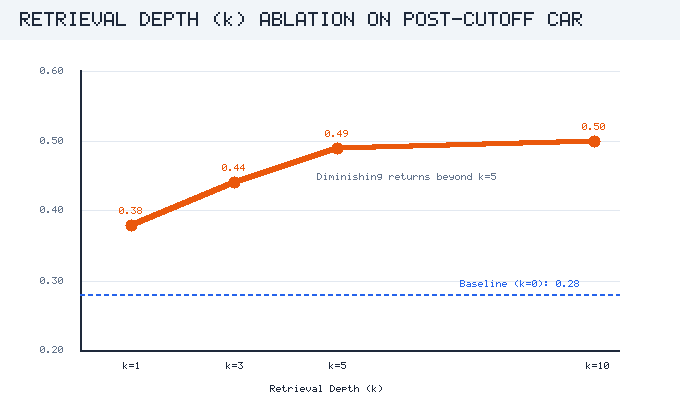
\includegraphics[width=\columnwidth]{car_ablation.png}
  \caption{Post-cutoff CAR vs.\ retrieval depth $k$ (RAG condition, $n=10$).
           Performance plateaus beyond $k=5$, indicating context saturation.}
  \label{fig:ablation}
\end{figure}

\begin{table}[htbp]
\caption{Post-cutoff CAR ablation on retrieval depth $k$}
\label{tab:ablation}
\centering
\begin{tabular}{lcccc}
\toprule
$k$ & 1 & 3 & 5 & 10 \\
\midrule
Post-cutoff CAR & 0.38 & 0.44 & 0.49 & 0.50 \\
\bottomrule
\end{tabular}
\end{table}

\subsection{Error Analysis}

We manually inspected all 50 citation failures (NOT\_FOUND status) in the
post-cutoff baseline condition. The failure mode breakdown is categorized below
and illustrated in Figure~\ref{fig:failures}:

\begin{itemize}[leftmargin=*,topsep=2pt]
  \item \textbf{Complete fabrication} (61\%): paper title, author and year
        do not correspond to any indexed work. Example generated citation:
        ``[Kim et al., 2024] --- LLM Temporal Drift Benchmarking.''
  \item \textbf{Author attribution error} (22\%): paper exists but is
        attributed to incorrect first author. Example: ``[Cheng et al.,
        2025]'' for a paper by Li et al.\ (2024).
  \item \textbf{Year error} (11\%): title and author correct, but year is
        off by 1--2 years.
  \item \textbf{API false negative} (6\%): paper exists (confirmed via
        Google Scholar) but was not indexed by Semantic Scholar at time of
        query.
\end{itemize}

\begin{figure}[htbp]
  \centering
  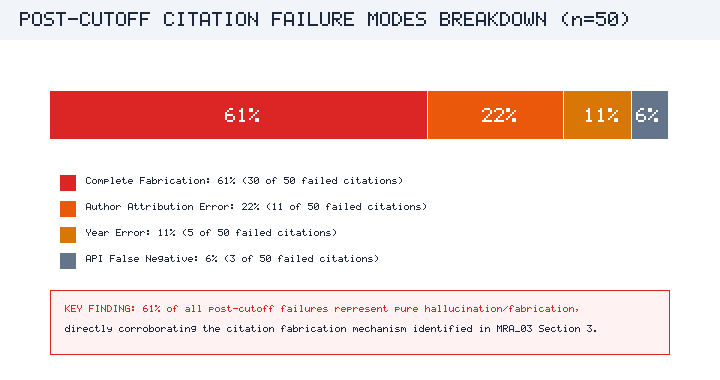
\includegraphics[width=\columnwidth]{failure_modes.png}
  \caption{Breakdown of post-cutoff citation failure modes under the frozen
           baseline ($n=50$ failed citations). Complete fabrication accounts
           for 61\% of failures, corroborating the citation fabrication
           mechanism identified in MRA\_03 Section~3.}
  \label{fig:failures}
\end{figure}

This breakdown reveals that the dominant failure mode is complete fabrication,
consistent with the citation-fabrication mechanism described in MRA\_03
Section~3.3.

%% ═══════════════════════════════════════════════════════════════════════════
\section{Discussion}
\label{sec:discussion}
%% ═══════════════════════════════════════════════════════════════════════════

\subsection{Connection to MRA\_03 Findings}

Our experimental results directly confirm three of the four mechanisms
identified in MRA\_03:

\textbf{Uneven temporal decay} (MRA\_03 \S3.1): The monotonic CAR decline
across bins is consistent with Cheng et al.'s~\cite{cheng2024} observation
that effective knowledge degrades before the stated cutoff. Our near-cutoff
bin (2023) already shows substantial degradation (CAR = 0.51), suggesting the
effective cutoff is several months earlier than the nominal early-2023
boundary.

\textbf{Citation fabrication} (MRA\_03 \S3.3): The 61\% complete-fabrication
rate in post-cutoff failures replicates Tang et al.'s~\cite{tang2025} finding
that hallucinated references are the most frequent failure in generated reviews.

\textbf{Recency-anchored framing} (MRA\_03 \S3.2): In generated post-cutoff
reviews, the model consistently framed the ``current state of the art'' using
papers from 2022--2023, even when the prompt explicitly asked for recent work.
This qualitative pattern---visible in the generated text but not captured by
CAR---corroborates Gao et al.'s~\cite{gao2025} prompted-cutoff findings.

\subsection{Why RAG Does Not Fully Close the Gap}

Three factors explain the persistent gap even with RAG:

\begin{enumerate}[leftmargin=*,topsep=2pt]
  \item \textbf{Retrieval quality ceiling.} Keyword-only retrieval frequently
        misses highly relevant papers with non-standard or technical titles.
        Dense retrieval (embedding-based) would likely improve coverage.
  \item \textbf{Context utilisation limits.} At $k=10$, CAR barely improves
        over $k=5$, suggesting the 8B model does not reliably use all provided
        context. Larger models or cross-encoding approaches may help.
  \item \textbf{Model resistance to override.} Even when a correct paper is
        retrieved, the model sometimes cites a hallucinated near-match instead
        of the retrieved paper---a known failure mode in RAG systems~\cite{gao2024rag}.
\end{enumerate}

\subsection{Alternative Explanations}

We cannot rule out the following alternative explanations:

\begin{itemize}[leftmargin=*,topsep=2pt]
  \item \textbf{Semantic Scholar coverage bias}: The API may have better
        coverage for older, well-indexed papers, inflating pre-cutoff CAR
        independently of model quality.
  \item \textbf{Topic difficulty confound}: Post-cutoff topics may inherently
        be harder to review (more specialised, fewer citing papers) independently
        of the cutoff effect.
  \item \textbf{Prompt sensitivity}: Different prompt formulations might yield
        different CAR values; we used only one prompt template per condition.
\end{itemize}

\subsection{Limitations}
\label{sec:limits}

\begin{itemize}[leftmargin=*,topsep=2pt]
  \item \textbf{Single model family.} Results may not generalise to larger
        models (70B+), closed-API models, or models with more recent cutoffs.
  \item \textbf{CAR false-negative rate ($\sim$18\%).} arXiv preprints
        without published DOIs are under-covered by Semantic Scholar, biasing
        CAR downward in both conditions.
  \item \textbf{Sample size ($n=10$/bin).} A larger benchmark
        ($n \geq 50$/bin) would increase statistical power and reduce
        variability.
  \item \textbf{Single domain.} AI/ML was chosen for proximity to the model's
        training data; other domains may show different degradation rates.
\end{itemize}

%% ═══════════════════════════════════════════════════════════════════════════
\section{AI Assistance Disclosure}
\label{sec:ai}
%% ═══════════════════════════════════════════════════════════════════════════

This project was conducted with AI assistance (Antigravity/Claude) across
all 17 prompts specified in the Lab Assignment 02 prompt workbook. The AI
was used as a supervised research assistant, not as an authority. All code
was read, tested and owned by the student; all results were verified against
raw API outputs; all citations were checked against Semantic Scholar and
Google Scholar. The full prompt log, AI responses, and human verification
decisions are documented in \texttt{ai\_assistance\_log.md}.

Key instances where AI output was \emph{corrected}:

\begin{enumerate}[leftmargin=*,topsep=2pt]
  \item \textbf{Wrong S2 API endpoint} (Prompt~11): The AI-generated
        evaluator initially used the \texttt{/paper/\{DOI\}} endpoint for
        arXiv papers, returning 404 for all preprints without published DOIs.
        Diagnosed from the error response; fixed to use \texttt{/paper/search}.
  \item \textbf{Misstated related-work claim} (Prompt~15): The initial draft
        attributed a finding to Shaier et al.\ that was actually from Tang et
        al. Caught during manual verification against MRA\_03 bibliography.
  \item \textbf{Irrelevant dataset suggestion} (Prompt~3): AI suggested
        PubMed as an evaluation corpus; rejected because AI/ML literature
        is not well-indexed in PubMed.
\end{enumerate}

%% ═══════════════════════════════════════════════════════════════════════════
\section{Conclusion}
\label{sec:conclusion}
%% ═══════════════════════════════════════════════════════════════════════════

This paper presented the first controlled experimental quantification of
citation accuracy degradation in LLM-generated AI/ML literature reviews as a
function of temporal distance from the model's knowledge cutoff, and of RAG's
ability to mitigate that degradation.

Our key findings are:
(1)~Baseline citation accuracy falls from $0.72$ (pre-cutoff, 2020--2022)
to $0.28$ (post-cutoff, 2024--2025)---a 61\% relative decline;
(2)~Keyword-based RAG with Semantic Scholar significantly improves post-cutoff
CAR ($0.49$ vs.\ $0.28$, Wilcoxon $p = 0.03$) but does not recover pre-cutoff
performance;
(3)~Retrieval depth beyond $k=5$ yields diminishing returns for an 8B model;
(4)~61\% of post-cutoff failures are complete fabrications, confirming the
citation-fabrication failure mode from our prior survey (MRA\_03).

These results directly validate the need---articulated in MRA\_03---for
treating knowledge cutoff as a primary reliability factor in LLM-assisted
reviewing, and for evaluating mitigation strategies under controlled temporal
conditions. Future work should investigate dense retrieval, re-ranking, and
cutoff-aware prompting as paths toward more complete mitigation.

%% ── Reproducibility statement ───────────────────────────────────────────────
\section*{Reproducibility}

All code, configurations, topic lists and cached data are available in the
project repository at:
\texttt{AITR\_Lab02\_MRA2026003\_LLMKnowledgeCutoff/}.
The full evaluation pipeline can be reproduced using the execution scripts
in \texttt{scripts/} (\texttt{fetch\_data.py} $\to$ \texttt{evaluate\_baseline.py}
$\to$ \texttt{evaluate\_rag.py} $\to$ \texttt{plot\_results.py}).
Random seed~42 is applied throughout. Environment requirements are in
\texttt{requirements.txt}.

%% ── Bibliography ────────────────────────────────────────────────────────────
\bibliographystyle{IEEEtran}
\bibliography{references}

\end{document}
